
\section{Equation Discretization and PISO Algorithm}\label{appendix 3}

\begin{figure}[h]
 \centering
\begin{tabular}{cc}
 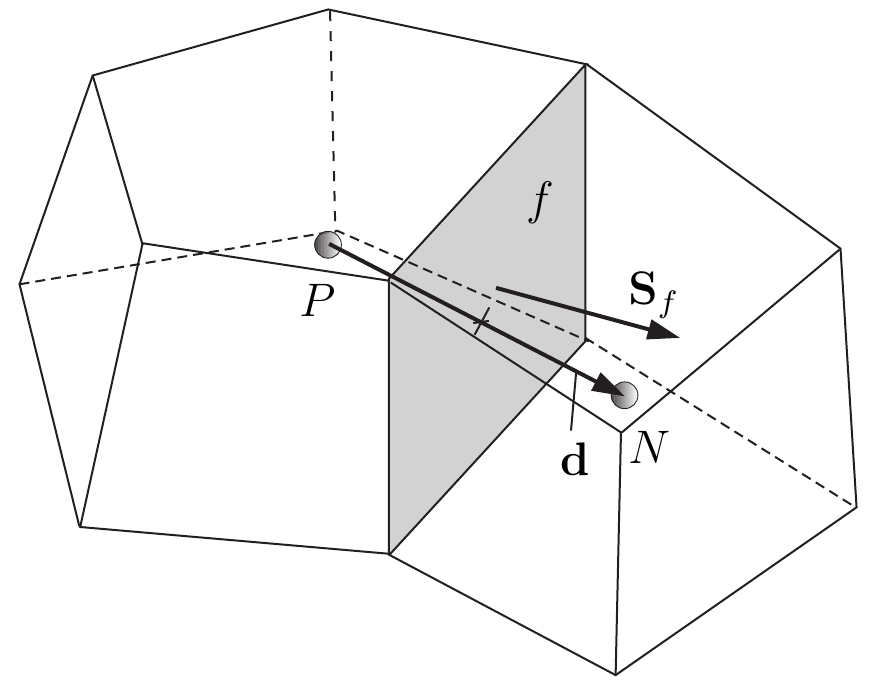
\includegraphics[width=0.55\textwidth]{./figuras/appA3/finite_volume.png}
\end{tabular}
 \caption{Finite volume discretization, reproduced from \cite{foamDev}.}
 \label{fig: fvm}
\end{figure}

A brief explanation of PISO algorithm and equation discretization as used in this work is here presented. The notation of equations follow OpenFOAM formulation explained in \cite{jasak}.

Superscripts \textbf{o} and \textbf{n} denote values from previous and current time-steps, respectively. \textbf{*} and \textbf{**} subscripts are used to denote intermediate fields computed before the final value of the time-step.

Subscripts \textbf{P} and \textbf{N} denote values stored in the center of owner and neighbor cells.  See Figure \ref{fig: fvm} for the geometric representation of two neighboring cells.

Subscript \textbf{f} indicates values interpolated from cell center to a face center. Advective terms were interpolated using the simple upwind scheme. The linear scheme was used for remaining interpolations. Setup of \verb|fvSchemes| input file is presented after PISO algorithm.

\clearpage
\textbf{Beginning of a new time-step:}
\begin{itemize}
  \item Evolve spray: move droplets and compute new spray source terms using old gas properties.

  \item Solve continuity equation for first density estimate $\bar{\rho}^{*}$:
    \begin{equation}
      \frac{\bar{\rho}^{*}-\bar{\rho}^{o}}{\Delta t} V_P +\sum_f F^{o} = S_m V_P \, ,
    \end{equation}
    where $F^{o}$ is the mass flow through cell faces from previous time-step:
  \begin{equation}
    F^{o}=\left(\bar{\rho}^{o}\tilde{\bv{U}}^{o}\right)_f\cdot \bv{S}_f \, .
  \end{equation} 
  This equation provides an explicit formulation for $\bar{\rho}^{*}$.

  \item Solve momentum equation for first velocity estimate $\bv{U}^{*}$ (momentum predictor):
    \begin{equation}
      \frac{\bar{\rho}^{*}\tilde{\bv{U}}^{*}-\bar{\rho}^{o}\tilde{\bv{U}}^{o}}{\Delta t} V_P + \sum_f F^{o}\tilde{\bv{U}}_f^{*} = \sum_f \bv{\tilde{\tau}}_f \cdot \bv{S}_f+\left(\bar{\rho}^{*}\bv{g}+\bv{S}_{mom} \right)V_P - \sum_f \bar{p}_{2,f}^{o}\bv{S}_{f}
    \end{equation}
    where 
    \begin{equation}
    \tilde{\bv{\tau}}=\underbrace{\sum_f \left( \mu_{eff}\nabla\tilde{\bv{U}}^{*} \right)_f \cdot \bv{S}_f}_{\text{implicit}} - \underbrace{\sum_f \mu_{eff,f}\left[\nabla \bv{\tilde{U}}^{o,T} -\frac{2}{3}\left(\nabla\cdot\tilde{\bv{U}}^{o}\right)\bv{I}\right]_f \cdot \bv{S}_f}_{\text{explicit}}
    \end{equation}
    The equation may be rewritten in a reduced semi-discretized form as:
    \begin{equation}
      \tilde{\bv{U}}_P^{*} = \frac{1}{a_P}\bv{H}(\tilde{\bv{U}}^{o})-\frac{1}{a_P}\nabla \bar{p}_2 \, .
    \end{equation}
    
  \item Solve species equation for $\tilde{Y}^{n}_k$:
  \begin{equation}
    \frac{\bar{\rho}^{*}\tilde{Y}_k^{n}-\bar{\rho}^{o}\tilde{Y}_k^o}{\Delta t} V_P +\sum_f F^{o}\tilde{Y}_{k,f}^{n} = \sum_f \left(\mu_{eff}\nabla\tilde{Y}_{k}^{n}\right)_f \cdot \bv{S}_f + S_{Yk} V_P
  \end{equation}

  \item Solve enthalpy equation for $\tilde{h}_{s}^{n}$:
  \begin{equation}
    \frac{\bar{\rho}^{*}\tilde{h}_s^{n}-\bar{\rho}^{o}\tilde{h}_s^o}{\Delta t} V_P +\sum_f F^{o}\tilde{h}_{s,f}^{n} = \sum_f \left(\mu_{eff}\nabla\tilde{h}_{s}^{n}\right)_f \cdot \bv{S}_{f}  + S_{hs} V_P
  \end{equation}
\end{itemize}

The computation of new pressure ($\bar{p}^n$) and velocity ($\bv{\tilde{U}}^n$) fields is performed in a iterative manner shown in next page.

\begin{tabular}{|p{0.95\textwidth}|} \hline
\textbf{PISO Loop (pressure-velocity coupling)} \\
\hline
Update $\rho$ with state equation using new temperature: $\bar{\rho}^{**} = p_0 \tilde{W} / R \tilde{T}^{n}$ \, ;\\
Compute second estimate of velocity ($\bv{U}^{**}$) without pressure contribution:
\begin{equation}
\tilde{\bv{U}}_P^{**} = \frac{1}{a_P}\bv{H}(\tilde{\bv{U}}^{*}) \, ;
\end{equation}

Update mass flow through cell faces using new density and velocity:
\begin{equation}
F^{*}=\left(\bar{\rho}^{**}\tilde{\bv{U}}^{**}\right)_f\cdot \bv{S}_f \, ;
\end{equation}

Solve pressure equation for the new dynamic pressure field $\bar{p}_2^n$:
\begin{equation}
  \sum_f \left[ F^{*} - \bv{S}_f\cdot\left(\frac{\bar{\rho}^{**}}{a_P}\nabla \bar{p}_2^{n} \right)_f \right] = S_m V_P \, ;
\end{equation}

Solve continuity equation for new density ($\bar{\rho}^n$) with $F^{*}$:
\begin{equation}
\frac{\bar{\rho}^{n}-\bar{\rho}^{o}}{\Delta t} V_P +\sum_f F^{*} = S_m V_P \, ;
\end{equation}

Compute the new velocity ($\tilde{\bv{U}}^{n}$) adding pressure contribution (momentum-corrector) and update mass fluxes:
\begin{equation}
\tilde{\bv{U}}^{n} = \tilde{\bv{U}}^{**} - \frac{1}{a_P}\sum_f \bar{p}_{2,f}^{n}\bv{S}_f \, ,
\end{equation}
\begin{equation}
 F^{n}=\left(\bar{\rho}^{n}\tilde{\bv{U}}^{n}\right)_f\cdot \bv{S}_f \, .
\end{equation}\\
\hline
\end{tabular}
PISO loop may be repeated inside the same time-step by setting $\tilde{\bv{U}}^{n}=\tilde{\bv{U}}^{o}$ and performing all steps again.

\clearpage
\begin{singlespace}
Setup of discretization schemes in \verb|fvSchemes| input file:
\begin{verbatim}
/*--------------------------------*- C++ -*----------------------------------*\
| =========                 |                                                 |
| \\      /  F ield         | OpenFOAM: The Open Source CFD Toolbox           |
|  \\    /   O peration     | Version:  1.7.1                                 |
|   \\  /    A nd           | Web:      www.OpenFOAM.com                      |
|    \\/     M anipulation  |                                                 |
\*---------------------------------------------------------------------------*/
FoamFile
{
    version     2.0;
    format      binary;
    class       dictionary;
    location    "system";
    object      fvSchemes;
}
// * * * * * * * * * * * * * * * * * * * * * * * * * * * * * * * * * * * * * //

ddtSchemes
{
    default         Euler;
}

gradSchemes
{
    default         none;

    //pEqn.H, velocity correction in PISO.
    grad(pd)         Gauss linear;
    
    // strain tensor
    grad(U)			Gauss linear;
}

divSchemes
{
    default         none;
    div(phi,rho)    Gauss upwind;
    div(phi,U)      Gauss upwind;
    div(phi,k)      Gauss upwind;
    div(phi,epsilon) Gauss upwind;
    div(phi,Yi_h)   Gauss upwind; // divergent scheme for Yk and hs
    div((muEff*dev2(grad(U).T()))) Gauss linear;
}

laplacianSchemes
{
    default         none;
    
    //UEq.H
    laplacian(muEff,U) Gauss linear uncorrected;
    
    //YEq.H
    laplacian(muEff,aC3H6O) Gauss linear uncorrected;
    laplacian(muEff,N2) Gauss linear uncorrected;
    laplacian(muEff,O2) Gauss linear uncorrected;
    laplacian(muEff,CO2) Gauss linear uncorrected;
    laplacian(muEff,H2O) Gauss linear uncorrected;
    
    //hsEq.H
    laplacian(alphaEff,hs) Gauss linear uncorrected;
    
    //pEq.H
    laplacian((rho*(1|A(U))),pd) Gauss linear uncorrected;
    
    //epsEq <kEpsilon.C>
    laplacian(DepsilonEff,epsilon) Gauss linear uncorrected;
    
    //kEq <kEpsilon.C>
    laplacian(DkEff,k) Gauss linear uncorrected;
}

interpolationSchemes
{
    default         linear;
    interpolate(HbyA) linear;
}

snGradSchemes
{
    default         uncorrected;
}

fluxRequired
{
    default         no;
    pd;
}
// * * * * * * * * * * * * * * * * * * * * * * * * * * * * * * * * * * * * * //
\end{verbatim}
\end{singlespace}
